\vspace{-2mm}
\section{Indexing}
\label{sec:index}
Indexing is important for the efficient processing of spatial queries
and analytics, especially for multi-dimensional spatial data and
complex spatial queries such as $\knn$ and spatial joins. In
particular, indexing is a critical component towards building an
effective optimizer in \name. Since \name is an in-memory analytical
engine, hence, reducing disk IOs is not a main focus of
indexing. Rather, the main objective of indexing in \name is to reduce
query latency via reducing cpu costs, and improve the over query
throughput in the system. For example, indexing helps prune irrelevant
RDD partitions (to an input query) which frees more cpu resources for
the underlying Spark engine, leading to higher query
throughput. Spatial indexing also helps speed up query processing for
complex queries such as $\knn$ and spatial joins. For example, Spark
and Spark SQL have to execute a $\knn$ join through cartesian product
between two (RDD) tables which is very expensive and not scalable,
whereas \name is able to process a $\knn$ join through distributed
R-tree index over the RDDs and dramatically reduce the query latency.

% Spark SQL claims that indexing is less important due to its in-memory
% computational model. However, it is not true when dealing with
% multi-dimensional data. For example, to process a $k$NN query, we need
% to calculate distances from the query point to all data points, take
% $k$ points with minimum distances in each partition and merge them in
% the driver program when processing without indexes. Such procedure
% requires touching every record in the table, thus will take numerous
% computing resources in the cluster. In contrast, if we have indexes
% built on tables, we can leverage them to cut down useless computations
% and improve system performance.

\name builds spatial indexes directly on RDDs to help speed up query
processing.  In Spark SQL, tables are represented as RDDs of records
(i.e., \texttt{RDD[row]}). Hence, indexing records of a table becomes
the problem of indexing elements in an RDD. However, RDDs are designed
for sequential scan, and random access is not supported and is very
expensive as it may simply become a full scan on the RDD. An added
complexity is that we want to introduce indexing support {\em without
  changing the Spark core} for the reasons explained in Section
\ref{sec:overview}. To overcome these challenges, we change the
storage format for an indexed table, i.e., a new abstraction called
\texttt{IndexedRDD[row]}, and employ a two-level indexing
strategy. This indexing strategy can accommodate different index
structures to support different queries in \name.


\Paragraph{IndexedRDD.} Records from a table in Spark SQL are stored
as \texttt{Row} objects and tables are stored as RDDs of \texttt{Row},
hence a table is stored as \texttt{RDD[row]} which may have many
partitions. To add index support over these records, we pack all
records (i.e. \texttt{Row} objects) within a RDD partition into an
array, which gives each record an unique subscript as its index. This
change also makes random access inside a RDD partition an efficient
operation with $O(1)$ cost. In particular, we introduce the
\texttt{IPartition} data structure:

\begin{lstlisting}[language=java]
case class IPartition[Type](Data: Array[Type], I: Index),
\end{lstlisting}\vspace{-1mm}
where \texttt{Index} is an abstract scala class we have designed and
it is instantiated with the following implementations:
\texttt{HashMap} (a hash index), \texttt{TreeMap} (a one dimension
index), and \texttt{RTree} (a multi-dimension index). Finally,
\texttt{IndexedRDD[Row]} is defined as \texttt{RDD[IPartition[Row]]},
when setting \texttt{Type=Row}:
\begin{lstlisting}[language=java]
type IndexedRDD[Type] = RDD[IPartition[Type]],
\end{lstlisting}\vspace{-1mm}
where the set of records from a table is partitioned into a set of
IPartition objects through the {\em partitioner} that will be
described next.

Each IPartition object represents a {\em local index} over records in
that partition. Furthermore, each IPartition object emits the
partition boundary information to construct a {\em global index}. That
being said, index construction in \name consists of three phases:
\emph{partition}, \emph{local index}, and \emph{global index}, as
shown in Figure \ref{fig:index}.

\begin{figure}[t!]
	\centering
	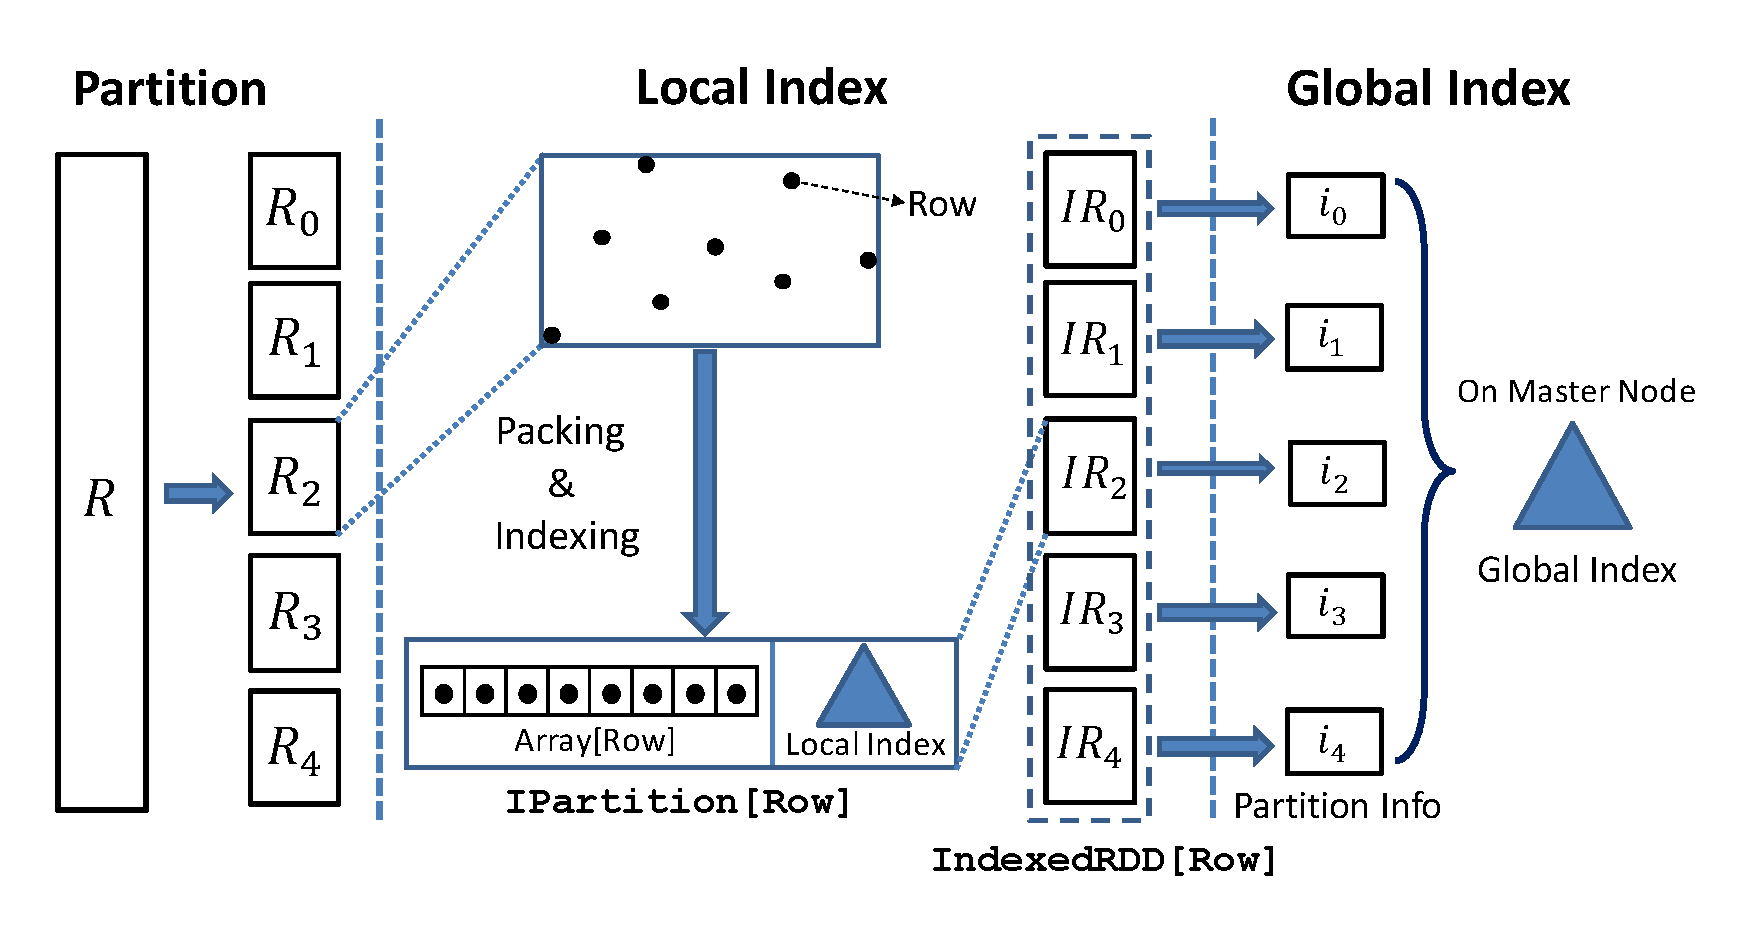
\includegraphics[width=3.4in]{figs/index}
	\vspace{-8mm}
	\caption{Two-level indexing strategy in \name.}
	\label{fig:index}
    \vspace{-4mm}
\end{figure}


\Paragraph{Partition.} The partition phase uses a {\em partitioner} to
partition a table of input data. The partitioner is an abstract class
that can be instantiated with different implementations on the
following key modules: (1) \emph{Partition Size.} Each partition
should have a proper size so as to avoid memory overflow. (2)
\emph{Data Locality.}  Records that locate close to each other (with
respect to the indexing attributes) should be assigned to the same
partition. (3) \emph{Load Balancing.} Partitions should be roughly of
the same size.

Spark allows users to define the partition strategy by implementing an
abstract class called \texttt{Partitioner}. A customized partitioner
should specify how many partitions it will generate and how an element
map to a according to its partition key. Spark provides two predefined
partitioners, range partitioner and hash partitioner, which is
sufficient when the partition key is one dimensional, but does not fit
well to the multi-dimensional case.

To address this problem, we defined a new partitioner named
\texttt{STRPartitioner} in \name. \texttt{STRPartitioner} takes a set
of random samples from the RDD for the input table and runs the first
iteration of Sort-Tile-Recursive (STR) algorithm \cite{str} to
determine partition boundaries. Note that boundaries generated by the
STR algorithm are minimum bounded rectangles (MBRs) of the samples,
thus, we need to extend theses MBRs so that they can properly cover
the space of the original data set. Finally, according to these
extended boundaries, \texttt{STRPartitioner} specifies the partition
that each record belongs to.

Note that \name makes no restriction as what partition strategy users
want to use. Instead of using the \texttt{STRPartitioner}, the end
user can always supply his/her own partitioner to \name. We choose the
\texttt{STRPartitioner} as the default partitioner in \name due to its
simplicity and proven effectiveness by many existing studies. As shown
in Figure \ref{fig:index}, we assume a RDD for an input table $R$ is
partitioned into a set of partitions $\{R_1, \ldots, R_m\}$ by the
partitioner. The number of partitions, $m$, is determined by \name's
optimizer which is discussed in Section \ref{sec:opt}.

\Paragraph{Local index.} In this phase, \name builds a user-specified
index structure, e.g., \texttt{RTree}, as a \emph{local} index for
data in each partition $R_i$ for $i\in\{1, \ldots, m\}$. Meanwhile, we
also alter the storage format of the input RDD from \texttt{RDD[Row]}
to \texttt{IndexedRDD[Row]}, by converting the RDD partition (a
partition of RDD[Row]) for each partition $R_i$ to an IPartition[Row]
object, as show in Figure \ref{fig:index}. In particular, records in
$R_i$ are stored into the \texttt{Array[Row]} object in the
\texttt{IPartition[Row]} object for $R_i$.

The \emph{local} index is built over the \texttt{Array[Row]} object
for each partition , and is co-located with \texttt{Array[Row]} object
within an \texttt{IPartition[Row]} object. The local index and the
local data from the partition's array of rows form the
\texttt{IPartition[Row]} object. As we can see, the storage format of
a table is no longer an RDD of \texttt{Row} objects, but an RDD of
\texttt{IPartition[Row]} objects, which by the definition above is an
\texttt{IndexedRDD} of \texttt{Row} objects. While packing partition
data and building local indexes, \name also collects several
statistics from each partition, such as number of records and
partition boundary, to facilitate the construction of the global
indexing as illustrated in Figure \ref{fig:index}.

Local indexes can be easily made persistent and fault tolerant, by
persisting the \texttt{IndexedRDD} (which is still a RDD object!) at
the \texttt{MEMORY\_AND\_DISK\_SER} storage level in Spark. This also
allows local indexes to be reused when data are loaded back into
memory from disk again, and avoids the rebuilding of partitions and
local indexes.

% By now, we finish local indexing for each partition and change
% storage format of the table from \texttt{RDD[Row]} to
% \texttt{RDD[PackedPartitionWithIndex]}.

\Paragraph{Global index.} The last phase of index construction is to
build a \emph{global} index which indexes all partitions. The global
index enables us to prune irrelevant partitions for an input query
{\em without invoking many workers} to look at data stored in
different partitions.

In this phase, partition boundaries generated by the partitioner and
other statistics collected in the local index phase are sent to the
{\em master node}. The master node utilizes these information to bulk
load an in-memory index which is stored in the {\em driver
  program}. Users may specify different types of global index. When
indexing one-dimensional data, a sorted array for the one dimensional
range boundaries is sufficient (the record count and other statistics
for each partition are also stored in each array element). In
multi-dimensional case, more complex index structures, such as R-Tree
\cite{rtree,DBLP:conf/sigmod/BeckmannKSS90} or KD-tree, which indexes
the MBRs for all partitions can be used. By default, \name keeps the
global indexes for different tables in the memory of the master node
at all time (i.e., in its driver program). But \name also allows users
to choose to persist the global indexes, and the corresponding
partition information and statistics to the file system.

\Paragraph{Fault tolerance.} By its construction, local indexes and
data in \name are {\em persisted automatically by the RDD abstraction
  of the Spark system}. Global indexes are kept in the heap space of
the driver program on the master node with no fault tolerance
guarantees by Spark. Nevertheless, global indexes can be lazily
reconstructed from partition boundaries and statistics collected from
persisted RDD when required, and as mentioned above, users can also
choose to persist them and then have the option of loading them back
from the file system.


%%% Local Variables:
%%% mode: latex
%%% TeX-master: "paper"
%%% End:
